\section{Statistique}

\subsection{Vocabulaire}

\begin{tabular}{c|c|c}

Vocabulaire ensembliste & Vocabulaire statistique & Vocabulaire probabiliste \\
\hline
Ensemble & Population & Univers \\
Sous-ensemble & Échantillon & Événement \\
Élément & Individu & Éventualité (cas possible) \\
Propriété & Caractère & {\Large $\times$} \\
\end{tabular} \\

% \textbf{Exemple} \\

\begin{center}

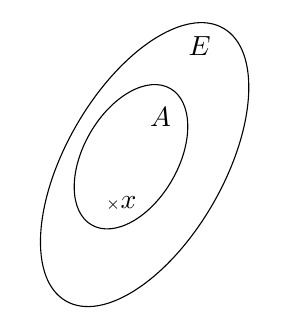
\begin{tikzpicture}
\begin{scope} [rotate=-30]
\draw (0,0)  circle  (1 and 2); 
\draw (0,0) ++(0:-.2) circle (.6 and 1); 
\end{scope} 
\draw (0.7,1.5) node {$E$} ; 
\draw (.2,.6) node {$A$} ; 
\draw (-.3,-.5) node {{\tiny $\times$} $\!\!x$} ; 
\end{tikzpicture}

$ A \subset E $, car A est un sous-ensemble de E.

$ x \in A $ et $ x \in E $ car $x$ est un élément de A, et par conséquent un élément de E. \\

\vspace*{2cm}


Il existe différents types de caractères : \\

\bigskip 
 
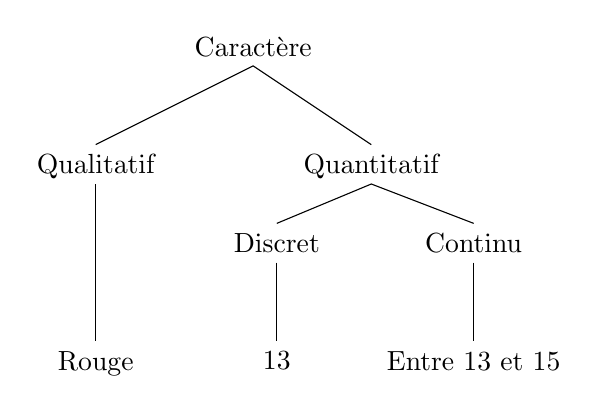
\begin{tikzpicture}
\draw(-2,2) node [below] {Qualitatif} -- (0,3) node [above] {Caractère} 
-- (1.5,2) node [below] {Quantitatif} ; 
\draw (-2,1.5) -- (-2,-.5) node [below] {Rouge} ; 
\draw (0.3,1) node [below]{Discret} -- (1.5,1.5) -- (2.8,1) node [below]{Continu} ; 
\draw (0.3,.5) -- (0.3,-.5) node [below]{13} ; 
\draw (2.8,.5) -- (2.8, -.5) node [below]{Entre 13 et 15} ; 
\end{tikzpicture}
\end{center} 

\newpage

\subsection{Étude d'un caractère quantitatif discret}

Population : Lycée International .

Echantillon : Les élèves d'une classe de Seconde.

Caractère : nombre de frères et sœurs

\subsubsection{Enquête}

\begin{tabular}{c|c}
Nombre de frères et sœurs & Nombre d'élèves \\
\hline
$0$ & $2$ \\
$1$ & $11$ \\
$2$ & $11$ \\
$3$ & $3$ \\
$4$ & $1$ \\
$5$ & $2$ \\
\end{tabular}

\subsubsection{Tableau}

Seront notés $x_i$ les valeurs du caractère et $n_i$ les effectifs correspondants.  \\

On notera $\Sigma_{n_i}$ la somme de tous nombres $n$ jusqu'à $n_i$, telle que : $\Sigma_{n_i} = n_1 + n_2 + n_3 + n_4 +$ ... $ + n_i $. \\

La colonne $p_i$ est la colonne des pourcentages. N'oublions pas que $p_i = \dfrac{n_i}{\Sigma_{n_i}}$. 

\begin{tabular}{c|c|c}
$x_i$ & $n_i$ & $p_i$ \\
\hline
$0$ & $2$ & $6,7$ \\
$1$ & $11$ & $36,7$ \\
$2$ & $11$ & $36,7$ \\
$3$ & $3$ & $10,0$ \\
$4$ & $1$ & $3,3 $\\
$5$ & $2$ & $6,7 $ \\
\hline
$\Sigma$ & $30$ & $100,1$ \\ 
\end{tabular} 

\medskip 

\textbf{N.B. : } $\mathbf{\Sigma_{p_i} = 100}$\textbf{. Ici, }$\mathbf{\Sigma_{n_i} = 100,1}$\textbf{ à cause d'un problème d'arrondi. } 

\newpage 

\subsubsection{Diagramme en bâtons des effectifs}

\smallskip 

\begin{center}

\begin{tikzpicture}[scale=.57]
    \tkzInit[xmax=7,ymax=11]
%    \tkzAxeXY
    \tkzGrid
    \tkzLabelX[orig=false, color=white]
    \tkzLabelY[orig=false]
    \tkzBardiagram[wd = 0.1,
                   pos = {below,outer sep = 5pt},
                   sp = 1,
                   noval]
          {
            0/2,
            1/11,
            2/11,
            3/3,
            4/1,
            5/2}
            \draw (13,9) node{\large Diagramme en bâtons des effectifs} ;  
\end{tikzpicture}
\end{center}

\subsection{Caractéristiques d'une série statistique correspondant à un caractère quantitatif continu}

\subsubsection{Le mode}

Le mode est la  valeur du caractère qui a le plus grand effectif. \\

\textbf{Exemple}

Les modes de la série statistique de la série précédente sont $1$ et $2$.

\subsubsection{L'étendue}

C'est la différence entre la plus grande valeur et la plus petite valeur du caractère. \\

\textbf{Exemple}

Dans la série statistique de la série précédente, l'étendue est $5 - 0 = 5$.

\subsubsection{La médiane}

Si elle existe, la médiane est la valeur du caractère qui partage l'effectif total en deux parties de même effectif. \\

\textbf{Exemple n°1}

Notes classées par ordre croissant. \\

$ \underbrace{ 7 \, ; \,  8 \, ; \,  9 \, ; \,  9 \, ; \,  10 \, ; \,  10 \, ; \, } 11 \underbrace{\, ; \,  12 \, ; \,  13 \, ; \,  14 \, ; \,  14 \, ; \,  15 \, ; \,  17.} $ \\

$ N = \Sigma_{n_i} = 13$ \\

$N$ est impair. La médiale est donc le terme de rang $\dfrac{N+1}{2}$. 

Donc $med = 11$ \\

\textbf{Exemple n°2} \\

$ \underbrace{7 \, ; \,  7 \, ; \,  9 \, ; \,  9 \, ; \,  10 \, ; \,  11 \, ; \, } 12 \, ; \,  13 \underbrace{\, ; \,  13 \, ; \,  13 \, ; \,  14 \, ; \,  14 \, ; \,  15 \, ; \,  15.}$ \\

$ N = 14 $. \\

$N$ est pair. La médiane est donc la moyenne entre le terme de rang $\dfrac{N}{2}$ et celui de rang $\dfrac{N}{2} + 1$. \\
Donc $med = \dfrac{12 + 13}{2} = 12,5 $. 

\newpage 

\textbf{Exemple n°3} \\

D'après la série statistique de la partie II., on a : \\

$ \underbrace{0 \, ; \,  0 \, ; \,  1 \, ; \,  1 \, ; \,  1 \, ; \,  1 \, ; \,  1 \, ; \,  1 \, ; \,  1 \, ; \,  1 \, ; \,  1 \, ; \,  1 \, ; \,  1 \, ; \,  2 \, ; \, } 2 \, ; \,  2 \underbrace{\, ; \,  2 \, ; \,  2 \, ; \,  2 \, ; \,  2 \, ; \,  2 \, ; \,  2 \, ; \,  2 \, ; \,  2 \, ; \,  3 \, ; \,  3 \, ; \,  3 \, ; \,  4 \, ; \,  5 \, ; \,  5}.$ \\

$med = \dfrac{2 + 2}{2} = 2$. \\

Il est aussi possible de construire un tableau, ce qui donne : \\

\textbf{Exemple n°1} \\

\begin{tabular}{rc|c|c}
&$x_i$ & $n_i$ & effectifs cumulés croissants \\
\cline{2-4}
& $7$ & $1$ & $1$ \\
& $8$ & $1$ & $2$ \\
& $9$ & $2$ & $4$ \\
& $10$ & $2$ & $6$ \\
\textcolor{red}{med} & $11$ & $1$ & $\quad \; \; \; 7$ 
                  \textcolor{red}{\Large $\leftarrow$} \\
& $12$ & $1$ & $8$ \\
& $13$ & $1$ & $9$ \\
& $14$ & $2$ & $11$ \\
& $15$ & $1$ & $12$ \\
& $17$ & $1$ & $13$ \\
\cline{2-4}
& $\Sigma$ & $13$ & {\Large $\times$} \\ 
\end{tabular} \\

\hspace*{.5 cm}

% Ajouter les flèches.

$\dfrac{N + 1}{2} = 7 $ \\

\textbf{Exemple n°2} \\

\begin{tabular}{rc|c|c}
& $x_i$ & $n_i$ & effectifs cumulés croissants \\
\cline{2-4}
& $7$ & $2$ & $2$ \\
& $9$ & $2$ & $4$ \\
& $10$ & $1$ & $5$ \\
 & $11$ & $1$ & $6$\\
\multirow{2}{1cm}{\textcolor{red}{ $\left.\begin{array}{c}
\\
\mathrm {med}\\
\end{array} \right[$}}& $12$ & $1$ & $\quad \; \; \; 7$ \textcolor{red}{\Large $\leftarrow$} \\
& $13$ & $3$ & $\quad \; \; 10$ \textcolor{red}{\Large $\leftarrow$} \\
& $14$ & $2$ & $12$ \\
& $15$ & $2$ & $14$ \\
\cline{2-4}
& $\Sigma$ & $14$ & {\Large $\times$} \\ 
\end{tabular} \\

% Ajouter les flèches.

\hspace*{.5cm}

$ \dfrac{N}{2} = 7 $ et $ \dfrac{N}{2} + 1 = 8 $ \\

\newpage 

\textbf{Exemple n°3} \\

\begin{tabular}{cc|c|c}
&$x_i$ & $n_i$ & effectifs cumulés croissants \\
\cline{2-4}
 &$0$ & $2$  & $2$  \\
 &$1$ & $11$ & $13$  \\
\textcolor{red}{med} & $2$ & $11$ & 
                      $\quad 24$\textcolor{red}{\Large $\leftleftarrows$}\\
&$3$ & $3$  & $27$ \\
&$4$ & $1$  & $28$ \\
&$5$ & $2$  & $30$ \\
\cline{2-4}
& $\Sigma$ & $30$ & {\Large $\times$} \\ 
\end{tabular} \\

% Ajouter les flèches.

\hspace*{.5cm}

$ \dfrac{N}{2} = 15 $ et $ \dfrac{N}{2} + 1 = 16$. \\

\subsubsection{Les quartiles}

\begin{itemize}
\item[*] Le premier quatile $Q_1$ est la plus petite valeur du caractère telle qu'au moins 25\% des valeurs du caractère soient inférieures ou égales à ce nombre.
\item[*] Le troisième quartile $Q_3$ est la plus petite valeur du caractère telle qu'au moins 75\% des valeurs du caractère soient inférieures ou égales à ce nombre.
\end{itemize}

\vspace*{.3cm}

\textbf{N.B.} : Le deuxième quartile n'est autre que la médiane.

\vspace*{.3cm}

\textbf{Exemple n°1} \\



$ 7 \, ; \,  7 \, ; \,  8 \, ; \,  9 \, ; \,  10 \, ; \,  12 \, ; \,  13 \, ; \,  13 \, ; \,  15 \, ; \,  16 \, ; \,  17 \, ; \,  18.$ \\

$\Sigma_{n_i} = N = 12$ \\

$N$ est divisible par 4. Donc $Q_1$ est le terme de rang $\dfrac{N}{4}$, et $Q_3$ est le terme de rang $\dfrac{3N}{4}$. \\

Ainsi,  \\

\begin{itemize}
\item[*] $\dfrac{N}{4} = 3$, donc $Q_1 = 8$.
\\
\item[*] $ \dfrac{3N}{4} = 9$, donc $Q_3 = 15$.
\end{itemize}

\vspace*{.3cm}

\textbf{Exemple n°2} \\

$ 7 \, ; \,  7 \, ; \,  8 \, ; \,  9 \, ; \,  10 \, ; \,  12 \, ; \,  13 \, ; \,  13 \, ; \,  15 \, ; \,  16 \, ; \,  17 \, ; \,  18 \, ; \,  19.$ \\

$\Sigma_{n_i} = N = 13$ \\

$N$ n'est pas divisible par 4. Donc $Q_1$ est le terme de rang le premier nombre entier qui suit $\dfrac{N}{4}$, 

et $Q_3$ est le terme de rang le premier nombre entier qui suit $\dfrac{3N}{4}$. \\

Ainsi,  \\

\begin{itemize}
\item[*] $\dfrac{N}{4} = 3,25$, donc $Q_1$ est le terme de rang 4, et $Q_1 = 9$.
\\
\item[*] $ \dfrac{3N}{4} = 9,75$, donc $Q_3$ est le terùe de rang 10, et $Q_3 = 16$.
\end{itemize}

\vspace*{.3cm}

$ 7 \, ; \,  7 \, ; \,  8 \, ; \,  9 \, ; \,  10 \, ; \,  12 \, ; \,  13 \, ; \,  13 \, ; \,  15 \, ; \,  16 \, ; \,  17 \, ; \,  18.$ \\

$\Sigma_{n_i} = N = 12$ \\

$N$ est divisible par 4. Donc $Q_1$ est le terme de rang $\dfrac{N}{4}$, et $Q_3$ est le terme de rang $\dfrac{3N}{4}$. \\

Ainsi,  \\

\begin{itemize}
\item[*] $\dfrac{N}{4} = 3$, donc $Q_1 = 8$.
\\
\item[*] $ \dfrac{3N}{4} = 9$, donc $Q_3 = 15$.
\end{itemize}

\newpage

\textbf{On peut aussi faire des tableaux :}

%Y mettre les couleurs. J'ai écrit la légende...

En orange l'« affichage machine », en rouge les quartiles et en vert la médiane. \\

Sur l'exemple n°1 : \\

On a $\dfrac{N}{4} = 3$, et $\dfrac{3N}{4} = 9$. De plus, $\dfrac{N}{2} = 6$ et $\dfrac{N}{2} + 1 = 7$.

\begin{tabular}{rrc|c|c}
& & $x_i$ & $n_i$ & Effectifs cumulés croissants \\
\cline{3-5}
\textcolor{DarkOrange}{$\mathrm{min}_{x}$}&   & 7 & 2 & 2 \\
\textcolor{DarkOrange}{$Q_1 = 8.5$}& \textcolor{Red}{$Q_1$}
    & 8 & 1 & $\quad$ 3 \textcolor{red}{$\leftarrow$}\\
& & 9 & 1 & 4 \\
& & 10 & 1 & 5 \\
% Les accollades par paire sinon le vert déteint
& \multirow{2}{2cm}{{\color{VertClair}
 $\left. \begin{array}{c}
          \mathrm{\fcolorbox{red}{white}{med=12.5}}\\
          \end{array}
  \right[$
 } }                  & 12 & 1 
           & $\quad$ 6 \textcolor{VertClair}{$\leftarrow$} \\
& & 13 & 2 & $\quad$ 8 \textcolor{VertClair}{$\leftarrow$}  \\
\textcolor{DarkOrange}{$Q_3 = 15.5$}
    &  \textcolor{Red}{$Q_3$}& 15 & 1 & $\quad$ 9 \textcolor{red}{$\leftarrow$} \\
& & 16 & 1 & 10 \\
& & 17 & 1 & 11 \\
\textcolor{DarkOrange}{$\mathrm{max}_x$}& & 18 & 1 & 12 \\
\cline{3-5}
& &  $\Sigma$ & 12 & {\Large $\times$} \\
& &  &\textcolor{DarkOrange}{n}& \\
\end{tabular}

\vspace*{.5cm}

Sur l'exemple n°2 : \\

On a $\dfrac{N}{4} = 3,25$, et $\dfrac{3N}{4} = 9,75$. De plus, $\dfrac{N+1}{2} = 7$.

\begin{tabular}{rrc|c|c}
&&$x_i$ & $n_i$ & Effectifs cumulés croissants \\
\cline{3-5}
\textcolor{DarkOrange}{$\mathrm{min}_{x}$} & & 7 & 2 & 2 \\
&&8 & 1 & 3 \\
\textcolor{DarkOrange}{$Q_1 = 8.5$}& \textcolor{Red}{$Q_1$}
       & 9 & 1 & $\quad$ 4 \textcolor{red}{$\leftarrow$} \\
&&10 & 1 & 5 \\
&&12 & 1 & 6 \\
&\textcolor{VertClair}{med} & \fcolorbox{red}{white}{13} 
     & 2 & $\quad$ 8 \textcolor{VertClair}{$\leftarrow$}  \\
&&15 & 1 & 9 \\
\textcolor{DarkOrange}{$Q_3 = 15.5$}
    &  \textcolor{Red}{$Q_3$} & 16 & 1 
            &  $\quad$ 10 \textcolor{red}{$\leftarrow$} \\
&&17 & 1 & 11 \\
&&18 & 1 & 12 \\
\textcolor{DarkOrange}{$\mathrm{max}_x$}&&19 & 1 & 13 \\
\cline{3-5}
&&$\Sigma$ & 13 & {\Large $\times$} \\
& &  &\textcolor{DarkOrange}{n}& \\
\end{tabular}

\newpage

\subsubsection{Diagramme en boîte (ou boîte à moustaches)}

\textbf{Exemple n°1 :}

%Mettre le dessin.
 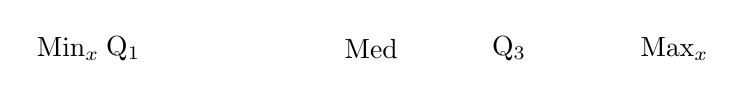
\begin{tikzpicture}[scale=0.7]
\tkzInit[xmax=20,xstep=1,ymax=2]
\tkzGrid [ultra thin,
% color=AntiqueWhite!10,sub,
color=AntiqueWhite,sub,
%       subcolor=AntiqueWhite!20,
       subxstep = 1](0,0)(20,2)
% \tkzLabelX[orig=false, color=white]
\tkzLabelX 
\tkzWhbox{7,8,12.5,15,18}
\draw (7,-1) node{$\mathrm{Min}_{x}$} ;  
\draw (8,-1) node{$\mathrm{Q}_{1}$} ;  
\draw (12.5,-1) node{Med} ; 
\draw (15,-1) node{$\mathrm{Q}_{3}$} ;   
\draw (18,-1) node{$\mathrm{Max}_{x}$} ;  
\end{tikzpicture}

% \bigskip

\textbf{Exemple n°2 :}

%Mettre le dessin.
 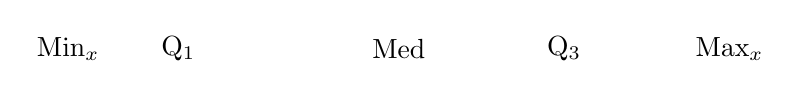
\begin{tikzpicture}[scale=0.7]
\tkzInit[xmax=20,xstep=1,ymax=2]
\tkzGrid [ultra thin,
% color=AntiqueWhite!10,sub,
color=AntiqueWhite,sub,
%       subcolor=AntiqueWhite!20,
       subxstep = 1](0,0)(20,2)
% \tkzLabelX[orig=false, color=white]
\tkzLabelX 

\tkzWhbox{7,9,13,16,19}
\draw (7,-1) node{$\mathrm{Min}_{x}$} ;  
\draw (9,-1) node{$\mathrm{Q}_{1}$} ;  
\draw (13,-1) node{Med} ; 
\draw (16,-1) node{$\mathrm{Q}_{3}$} ;   
\draw (19,-1) node{$\mathrm{Max}_{x}$} ;  

\end{tikzpicture}
% \newpage

\subsubsection{La moyenne}

\textbf{Exemple n°1} : Notes.

\begin{tabular}{c|c|c}
$x_i$ & $n_i$ & $n_ix_i$ \\
\hline
2 & 2 & 4	\\
6 & 7 & 42 \\
10 & 9 & 90 \\
14 & 9 & 126 \\
18 & 1 & 18 \\
\hline
$\Sigma$ & 28 & 280 \\
    & \textcolor{DarkOrange}{n} & \textcolor{DarkOrange}{$\Sigma x$} \\
\end{tabular}

\vspace{.3cm}

$\overline{x} = \dfrac{\Sigma_{n_ix_i}}{\Sigma_{n_i}} $ \\

$\overline{x} = \dfrac{280}{28} = 10 $

\newpage

\subsubsection{L'écart type}

\textbf{a) Introduction}

On observe les résultats en mathématique de 2 élèves, Sylvain et Sylvette, au cours d'un trimestre. On appelle « Élève A » Sylvain, et « Élève B », Sylvette. \\

\begin{itemize}
\item[*] Élève A : $ 11 / 9 / 13 $
\item[*] Élève B : $ 12 / 3 / 18 $
\end{itemize}

\vspace{.3cm}

On constate que $\overline{x_A} = \overline{x_B} = 11 $. \\

\centerline{\footnotesize
\begin{tabular}{c|c|c|c|c|c|c|c|c|c}
& Notes & Moyenne & Écarts & Moyenne & Valeurs & Moyenne & Carrés & Moyenne & Racine \\ 
& & & par & des & absolues & des & des & des & carrée \\
& & & rapport & écarts & des & valeurs & écarts & carrés & de la \\
& & & à la & par & écarts & absolues & par & des & moyenne \\
& & & moyenne & rapport & par & des & rapport & écarts & des \\
& & & & à la & rapport & écarts & à la & par & carrés \\
& & & & moyenne & à la & par & moyenne & rapport & des \\
& & & & & moyenne & rapport & & à la & écarts \\
& & & & & & à la & & moyenne & par \\
& & & & & & moyenne & & & rapport \\
& & & & & & & & & à la \\
& & & & & & & & & moyenne \\
\hline
& & & & & & & & & \\
Élève A & $11$ / $9$ / $13$ & $11$ & $0$ / $-2$ / $+2$ & $0$ & $0$ / $2$ / $2$ & $\dfrac{4}{3} \approx 1,33$ & $0$ / $4$ / $4$ & $\dfrac{8}{3} \approx 2,67$ & $\sqrt{\dfrac{8}{3}} \approx 1,63$ \\
& & & & & & & & & \\
Élève B & $12$ / $3$ / $18$ & $11$ & $+1$ / $-8$ / $+7$ & $0$ & $1$ / $8$ / $7$ & $\dfrac{16}{3} \approx 5,33$ & $1$ / $64$ / $49$ & $38$ & $\sqrt{38} \approx 6,16$ \\
%& & & & RATÉ, il aurait fallu faire une moyenne arithmétique, pas algébrique & & Pas mal, mais pas exploitable & & Ça n'a pas de signification, des points au carré & \\
\hline
& & & & & & & & & \\
& & & & & & & ÉCART-MOYEN & VARIANCE & ÉCART-TYPE \\
\end{tabular}}

\vspace*{.5cm}

\textbf{b) Définition :}

On note l'écart type $\sigma_x$, et on a : $ \sigma_x = \sqrt{\dfrac{\Sigma_{n_i}\left(x_i - \overline{x}\right)^2}{\Sigma_{n_i}}} $. \\

\textbf{c) Exemple :} \\

\begin{tabular}{c|c|c|c}
$x_i$ & $n_i$ & $n_ix_i$ & $n_i\left(x_i - \overline{x}\right)^2$ \\
\hline
2 & 2 & 4 & 128 	\\
6 & 7 & 42 & 112 \\
10 & 9 & 90 & 0 \\
14 & 9 & 126 & 144 \\
18 & 1 & 18 & 64 \\
\hline
$\Sigma$ & 28 & 280 & 448 \\
\end{tabular}

\vspace*{.3cm}

$ \overline{x} = \dfrac{\Sigma{n_ix_i}}{\Sigma_{n_i}} = \dfrac{280}{28} = 10 $ \\

\vspace*{.3cm}

$\sigma_x = \sqrt{\dfrac{448}{28}} = 4 $ \\

\newpage

\textbf{d) Autre formule} \\

$ \sigma_x^2 = \dfrac{\Sigma_{n_i \times \left(x_i - \overline{x}\right)^2}}{\Sigma_{n_i}} $ \\

$ \sigma_x^2 = \dfrac{\Sigma_{n_i \times x_i^2 - 2\overline{x}x_i + \overline{x}^2}}{\Sigma_{n_i}} $ \\

$ \sigma_x^2 = \dfrac{\Sigma_{n_ix_i^2} - 2\overline{x}\Sigma_{n_ix_i} + \overline{x}^2\Sigma{n_i}}{\Sigma_{n_i}} $ \\

$ \sigma_x^2 = \dfrac{\Sigma_{n_ix_i^2}}{\Sigma_{n_i}} - 2\overline{x} \dfrac{\Sigma_{n_ix_i}}{\Sigma_{n_i}} + \overline{x}^2 \dfrac{\Sigma_{n_i}}{\Sigma_{n_i}} $ \\

$ \sigma_x^2 = \overline{x^2} - 2\overline{x} \times \overline{x} + \overline{x}^2 \times 1 $ \\

$ \sigma_x^2 = \overline{x^2} - 2\overline{x}^2 + \overline{x}^2 $ \\

$ \sigma_x^2 = \overline{x^2} - \overline{x}^2 $

Et donc $ \sigma_x = \sqrt{\overline{x^2} - \overline{x}^2} $ \\

\textbf{e) Exemple :} \\

\begin{tabular}{c|c|c|c}
$x_i$ & $n_i$ & $n_ix_i$ & $n_ix_i^2$ \\
\hline
2 & 2 & 4 & 8 	\\
6 & 7 & 42 & 252 \\
10 & 9 & 90 & 900 \\
14 & 9 & 126 & 1764 \\
18 & 1 & 18 & 324 \\
\hline
$\Sigma$ & 28 & 280 & 3248 \\
\end{tabular}

\vspace{.3cm
}
On rapelle que $\overline{x} = 10 $. \\

On a : $ \sigma_x = \sqrt{\overline{x^2} - \overline{x}^2} = \sqrt{\dfrac{3248}{28} - \left(\dfrac{280}{28}\right)^2} = 4 $ \\

%On notera l'affiche machine en orange...

\newpage

\subsubsection{Répartition « normale »}

Soit $\left(x_i,n_i\right)$ une série statistique. 

Soient $\overline{x}$ la moyenne et $\sigma_x$ l'écart-type. \\

On considère que la répartition est « normale » : \\

\begin{itemize}
\item[*] si les valeurs du caractère comprises entre $\overline{x} - \sigma_x$ et $\overline{x} + \sigma_x$ représentent 68\% de l'effectif total.
\item[*] \textbf{ou} si les valeurs du caractère comprises entre $2\overline{x} - 2\sigma_x$ et $2\overline{x} + 2\sigma_x$ représentent 95\% de l'effectif total.
\item[*] \textbf{ou} si les valeurs du caractère comprises entre $3\overline{x} - 3\sigma_x$ et $3\overline{x} + 3\sigma_x$ représentent 99\% de l'effectif total.
\end{itemize}

\vspace*{.3cm}

%Mettre les dessin.

\pgfmathdeclarefunction{gauss}{2}{%
    \pgfmathparse{1/(#2*sqrt(2*pi))*exp(-((x-#1)^2)/(2*#2^2))}%
        }

\begin{tikzpicture}

    \begin{axis}[
      hide y axis, tick align=outside,
      domain=-4:4, samples=50,
%       axis lines*=left, xlabel=Gauss, ylabel=$~$,
        axis lines*=left, xlabel=$~$, ylabel=$~$,
      height=5cm, width=13cm,
      xtick={-4,-3,-1.5,-1,0,1,1.5,3,4}, ytick=\empty,
      xticklabels={%
        $\overline{x}-3\sigma_x$,
        $\overline{x}-2\sigma_x$,
        $\overline{x}-\sigma_x$,
        ,
        $\overline{x}$,
        ,
        $\overline{x}+\sigma_x$,
        $\overline{x}+2\sigma_x$,
        $\overline{x}+3\sigma_x$}      
      ]
   
      \addplot [fill=blue!30, domain=-1.5:1.5] {gauss(0,1)}\closedcycle;
         
            \addplot [thick,red,domain=-4:4] {gauss(0,1)};
   \addplot [red, domain=-4:4] {gauss(0,1)}\closedcycle;
   
         \addplot [thick,green,domain=-3:3] {gauss(0,1)};
      \addplot [fill=VertClair, domain=-3:-1.5] {gauss(0,1)}\closedcycle;   
      \addplot [fill=VertClair, domain=1.5:3] {gauss(0,1)}\closedcycle;

      \addplot [thick,black!50!black,domain=-1.5:1.5] {gauss(0,1)};

    \end{axis}
    
    \draw (5.7,1.5) node {68\%} ;  
    \draw [VertClair](10,3) node {$\bumpeq \; $ 95\%} ;    
    \draw [red](10,2.5) node {$\bumpeq \; $ 99\%} ; 
\end{tikzpicture}

Ceci est appelé « Courbe en cloche de Gauss ». \\

\textbf{Exemple} \\

Si $\overline{x} = 10$ et $ \sigma_x = 4$, alors :

\begin{itemize}
\item[*] $\overline{x} - \sigma_x = 6$ et $\overline{x} + \sigma_x = 14$. On a donc $7 + 9 + 9 = 25$ élèves, soit 89,3\%. 
\item[*] $2\overline{x} - 2\sigma_x = 2$ et $2\overline{x} + 2\sigma_x = 18$. On a donc $28$ élèves, soit 100\%. 
\end{itemize}

\newpage

\subsection{Exercice : Étude d'un caractère quantitatif discret}

Dans une maternité, on étudie la taille des bébés en cm pour 200 bébés. \\

\begin{tabular}{rc|c|c|c|c|c}
&\textcolor{DarkOrange}{\Ovalbox{$L_1$}}
          &\textcolor{DarkOrange}{\Ovalbox{$L_2$}}&&&&\\
 & $x_i$ & $n_i$ & $p_i$ & Effectifs cumulés croissants & $n_ix_i$ & $n_ix_i^2$ \\
\cline{2-7}
 \textcolor{DarkOrange}{$\mathrm{min}_{x}$} & 43 & 4 & 2 & 4 & 172 & 7 396 \\
 & 44 & 0 & 0 & 4 & 0 & 0 \\
 & 45 & 0 & 0 & 4 & 0 & 0 \\
 & 46 & 8 & 4 & 12 & 368 & 16 928 \\
 & 47 & 16 & 8 & 28 & 752 & 35 344 \\
 & 48 & 22 & 11 & 50 & 1056 & 50 688 \\
 & 49 & 38 & 19 & 88 & 1862 & 91 238 \\
 & 50 & 42 & 21 & 130 & 2100 & 105 000 \\
 & 51 & 30 & 15 & 160 & 1530 & 78 030 \\
 & 52 & 16 & 8 & 176 & 832 & 43 264 \\
 & 53 & 14 & 7 & 190 & 742 & 39 326 \\
 & 54 & 4 & 2 & 194 & 216 & 11 664 \\
 & 55 & 4 & 2 & 198 & 220 & 12 100 \\
 & 56 & 0 & 0 & 198 & 0 & 0 \\
 \textcolor{DarkOrange}{$\mathrm{max}_{x}$} & 57 & 2 & 1 & 200 & 114 & 6 498 \\
\cline{2-7}
 & $\Sigma$ & 200 & 100 & {\Large $\times$} & 9 964 & 497 476 \\
 &  & \textcolor{DarkOrange}{n} &\multicolumn{2}{c}{}   
 & \multicolumn{1}{c}{\textcolor{DarkOrange}{$\Sigma x$} } 
 &  \multicolumn{1}{c}{\textcolor{DarkOrange}{$\Sigma x^2$}}\\ 
\end{tabular}

\subsubsection{Mode et étendue}

\begin{itemize}
\item[*] Mode : $50$
\item[*] Etendue : $57 - 43 = 14$.
\end{itemize}

\medskip 

\begin{center}
\textbf{Diagramme en bâtons des pourcentages}

\begin{tikzpicture}[scale=.7]
    \tkzInit[xmin=42,xmax=57,ymax=22, ystep=2]

    \tkzGrid[color=AntiqueWhite]
    \tkzDrawX[label=$~$]
    \tkzLabelX[orig=false, color=black ]
   \tkzDrawY[label=$~$]
    \tkzLabelY[orig=false]
%     \tkzAxeXY
    \tkzBardiagram[wd = 0.1,
                   pos = {below,outer sep = 5pt},
                   sp = 1,
                   noval]
     { /2, /0, /0, /4, /8, /10.5, /19, /21, /17, /8, /7, /2, /2, /0, /1}
%            \draw (13,9) node{\large Diagramme en bâtons des effectifs} ;  
\end{tikzpicture}
\end{center}

\newpage 

\subsubsection{Médiane, 1$^{\mathrm {\bf er}}$ quartile et 3$^{\mathrm{\bf e}}$ quartile}

\textbf{Médiane} \\

$ N = 200 $. $N$ est un nombre pair. \\

$\dfrac{N}{2} = 100 $ et $\dfrac{N}{2} + 1 = 101 $. \\

\begin{itemize}
\item[*] Le terme de rang 100 est 50.
\item[*] Le terme de rang 101 est 50.
\end{itemize}

\vspace*{.3cm}

$\mathrm{med} = \dfrac{50 + 50}{2} = $ 
      \textcolor {DarkOrange}{\Ovalbox {\textcolor{black}{50}} med = 50}. \\

$\mathbf{Q_1}$ \textbf{et} $\mathbf{Q_3}$ \\

$ N = 200 $. $N$ est divisible par 4. \\

$\dfrac{N}{4} = 50 $ et $\dfrac{3N}{4} = 150 $. \\

\begin{itemize}
\item[*] Le terme de rang 50 est 48.
\item[*] Le terme de rang 150 est 51.
\end{itemize}

\vspace*{.3cm}

Donc $Q_1 = 48$ et $Q_3 = 51$. \\

\textbf{Boîte à moustaches}

\bigskip 

%Inclure le dessin.

 \begin{tikzpicture}[scale=0.7]
\tkzInit[xmin=42,xmax=58,xstep=1,ymax=2]
\tkzGrid [ultra thin,
% color=AntiqueWhite!10,sub,
color=AntiqueWhite,sub,
%       subcolor=AntiqueWhite!20,
       subxstep = 1](42,0)(58,2)
% \tkzLabelX[orig=false, color=white]
\tkzLabelX 

\tkzWhbox{43,48,50,51,57}
\draw (1,1.5) node{$\mathrm{Min}_{x}$} ;  
\draw (5.5,1.5) node{$\mathrm{Q}_{1}$} ;  
\draw (8,1.8) node{Med} ; 
\draw (9.5,1.5) node{$\mathrm{Q}_{3}$} ;   
\draw (15,1.5) node{$\mathrm{Max}_{x}$} ;  

\end{tikzpicture}

Interprétation de la médiane : \\

Environ 50\% des bébés mesurent moins de 50 cm. \\
Environ 50\% des bébés mesurent plus de 50 cm. \\

Interprétation de l'\underline{écart interquartile} : \\

Environ 50\% des bébés mesurent entre 48 et 51 cm. 

\newpage

\subsubsection{Moyenne et écart-type}

$\overline{x} = \dfrac{\Sigma_{n_ix_i}}{\Sigma_{n_i}} = \dfrac{9964}{200} = 49,82$. \\

Donc $\overline{x} = 49,82$cm. \\

$\sigma_x = \sqrt{\overline{x^2} - \overline{x}^2} = \sqrt{\dfrac{497476}{200} - \left(\dfrac{9964}{200}\right)^2} \approx 2,31$. \\

Donc $\sigma_x = 2,31$cm. \\

\subsubsection{Répartition « normale »}

\begin{itemize}
\item[*] $\overline{x} - \sigma_x = 47,51$. \\ $\overline{x} + \sigma_x = 52,13$. \\On a donc $22 + 38 + 42 + 30 + 16 = 148$ bébés, soit 74\%. 
\\
\item[*] $2\overline{x} - 2\sigma_x = 45,20$ \\ $2\overline{x} + 2\sigma_x = 54,44$. \\ On a donc $200 - 4 - 4 - 2 = 190$ bébés, soit 95\%. 
\end{itemize}

\newpage

\subsection{Étude d'un caractère quantitatif continu}

Échantillon : Les élèves d'une classe de Seconde. \\
Caractère : Notes en mathématique. \\

On regroupe les valeurs du caractère par \underline{classes d'amplitude} 4 : \\

\begin{tabular}{c|c|c|c}
Classes & $n_i$ & $p_i$ à l'unité & Pourcentages cumulés croissants \\
\hline
$[0,4[$ & 2 & 7 & 7 \\
$[4,8[$ & 7 & 25 & 32 \\
$[8,12[$ & 9 & 32 & 64 \\
$[12,16[$ & 9 & 32 & 96 \\
$[16,20]$ & 1 & 4 & 100 \\
\hline
$\Sigma$ & 28 & 100 & {\Large {$\times$}} \\
\end{tabular}

\subsubsection{Histogramme des pourcentages}

\begin{center}

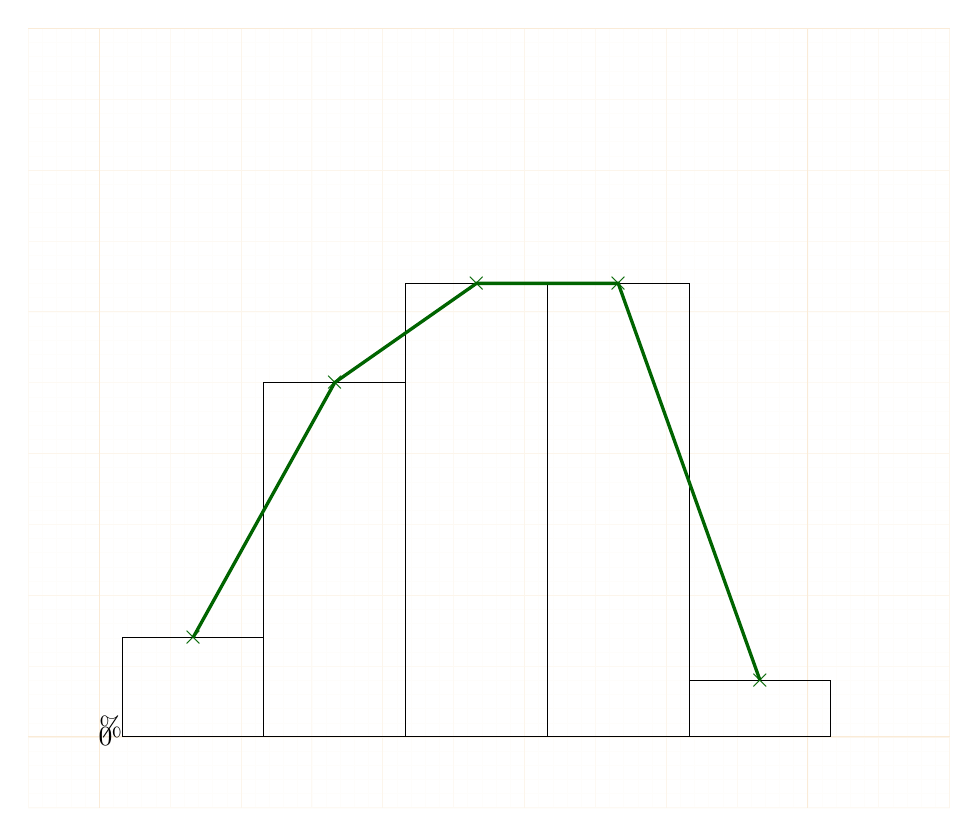
\begin{tikzpicture}[scale=1.8]
    \tikzstyle{AxeXStyle}=[>=latex’,->]
    \tikzstyle{AxeYStyle}=[-]
    \tkzInit[xmax=22,xstep=4,ymax=40,ystep=10]
    \tkzDrawX[label=$~$]
    \tkzLabelX[orig=false, color=black ]
    \tkzDrawY[label=$\%$]
    \tkzLabelY[orig=false, color=black ]  

% \tkzHistogram[noval, color=white] {7,25,32,32,4}
\draw  
(0,0) node [left] {\textcolor{black}{0}} -- (0,.7) -- (1,.7) -- (1,0) -- (1,2.5) -- (2,2.5) -- (2, 0) -- (2, 3.2) 
-- (3, 3.2) -- (3,0) -- (3,3.2) -- (4,3.2) -- (4, 0) 
-- (4,.4) -- (5,.4) -- (5,0) -- cycle ; 
\draw [line width=1.2, color=DarkGreen] (.5,.7) node {$\times$} -- (1.5,2.5)node {$\times$} -- (2.5,3.2) node {$\times$} -- (3.5,3.2) node {$\times$} -- (4.5,.4) node {$\times$} ; 

\begin{pgfonlayer}{background}  
% Attention l'ordre de ces lignes est important 
% Ne pas le modifier   
\draw[step=1mm,ultra thin,AntiqueWhite!10](-.5,-.5)  grid (6,5);
\draw[step=5mm,very thin,AntiqueWhite!30] (-.5,-.5)   grid (6,5);
\draw[step=1cm,very thin,AntiqueWhite!50] (-.5,-.5)   grid (6,5);
\draw[step=5cm,thin,AntiqueWhite]         (-.5,-.5)  grid (6,5);
\end{pgfonlayer} 
\end{tikzpicture}
\end{center}

En vert, le polygone des pourcentages.

\newpage

\subsubsection{Histograme des pourcentages cumulés croissants}

\begin{center}

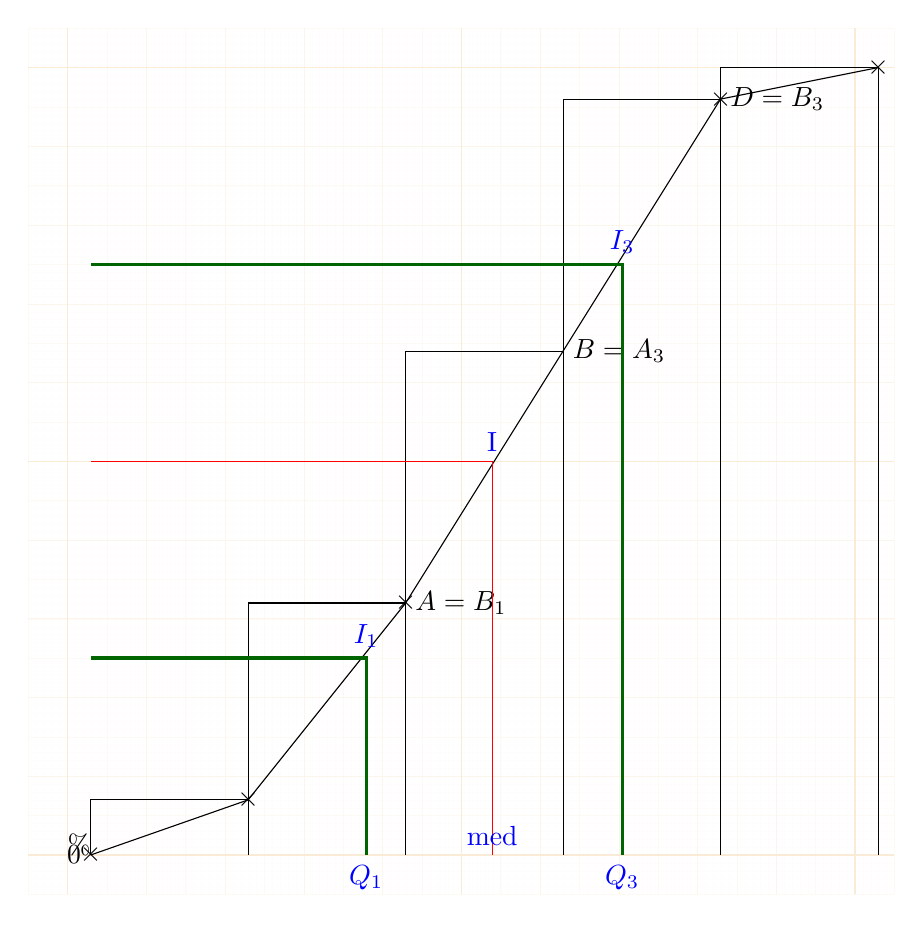
\begin{tikzpicture}[scale=1]
    \tikzstyle{AxeXStyle}=[>=latex’,->]
    \tikzstyle{AxeYStyle}=[-]
    \tkzInit[xmax=21,xstep=2,ymax=100,ystep=10]
    \tkzDrawX[label=$~$]
    \tkzLabelX[orig=false, color=black ]
    \tkzDrawY[label=$\%$]
    \tkzLabelY[orig=false, color=black ]  

\draw  (0,0) node {$\times$} -- (2,.7) node {$\times$} -- (4,3.2) node {$\times$} -- (8,9.6) node {$\times$} -- (10,10.0) node {$\times$} ; 

\draw (0,0) node [left] {$0$} -- (0,.7) -- (2,.7) -- (2,0) 
-- (2,3.2) -- (4,3.2) node [right] {$A=B_1$} -- (4,0) -- (4,6.4) -- (6, 6.4) node [right] {$B=A_3$} -- (6,0) 
-- (6, 9.6) -- (8,9.6) node [right] {$D=B_3$} -- (8, 0) -- (8,10) -- (10,10) -- (10,0) ; 

\draw[color=DarkGreen,line width=1.2] (3.5,0) node [below] {\textcolor{blue}{$Q_1$}} 
    -- (3.5, 2.5) node [above] {\textcolor{blue}{$I_1$}} 
    -- (0, 2.5) ;  
    
\draw[color=red] (5.1,0) node [above] {\textcolor{blue}{med}} 
    -- (5.1, 5) node [above] {\textcolor{blue}{I}} 
    -- (0,5) ;    

\draw[color=DarkGreen,line width=1.2] (6.75,0) node [below] {\textcolor{blue}{$Q_3$}} 
    -- (6.75, 7.5) node [above] {\textcolor{blue}{$I_3$}} 
    -- (0, 7.5) ; 
         
\begin{pgfonlayer}{background}  
% Attention l'ordre de ces lignes est important 
% Ne pas le modifier   
\draw[step=1mm,ultra thin,AntiqueWhite!10](-.5,-.5)  grid (10.5,10.5);
\draw[step=5mm,very thin,AntiqueWhite!30] (-.5,-.5)  grid (10.5,10.5);
\draw[step=1cm,very thin,AntiqueWhite!50] (-.5,-.5)  grid (10.5,10.5);
\draw[step=5cm,thin,AntiqueWhite]         (-.5,-.5)  grid (10.5,10.5);
\end{pgfonlayer} 
\end{tikzpicture}
\end{center}

Grâce au polygone des pourcentages cumulés croissants, on peut lire graphiquement : 

\begin{itemize}
\item[*] med $\approx 10,2$.
\item[*] $ Q_1 \approx 6,8$.
\item[*] $ Q_3 \approx 13,4$.
\end{itemize}

\vspace*{.3cm}

Par le calcul, on a : \\

\textbf{Médiane}

Avec les points $A(8,32) et B(12,64)$. \\

Équation de la droite $(AB)$ : $y=8x - 32$. \\

Intersection de $(AB)$ et la droite $y=50$. \\

$8x - 32 = 50$ \\

$ 8x = 82$ \\

$ x = 10,25 $ \\

Donc med $= 10,25$. 50\% des élèves ont eu moins de $10,25/20 $ et 50\% des élèves ont eu plus de $10,25/20$. \\

$\mathbf{Q_1}$  \\

Avec les points $A(8,32)$  et $C(4,7)$. \\

Équation de la droite $(AB)$ : $y=\dfrac{25}{4}x - 18 = 6,25x - 18$. \\

Intersection de $(AC)$ et la droite $y=25$. \\

$ 6,25x - 18 = 25$ \\

$ 6,25x = 43 $ \\

$ x = \dfrac{43}{6,25} = \dfrac{172}{25} $ \\

$ x \approx 6,88 $ \\

Donc $Q_1 = 6,88$. \\

$\mathbf{Q_3}$ \\

Avec les points $A_3(12,64)$  et $B_3(16,96)$. \\

%-----------

Équation de la droite $(AB)$ : $y= 8x - 32$.

Intersection de $(A_3B_3)$ et la droite $y=75$. \\

$ 8x - 32 = 75 $ \\

$ 8x = 107 $ \\

$ x = \dfrac{107}{8} = 13,375 $ \\

$ x \approx 13,38 $ \\

Donc $Q_1 = 13,38$. \\

50\% des élèves ont eu entre $6,88/20$ et $13,38/20$.

\newpage 

\subsubsection{Moyenne et écart-type}

 
% Inclure l'écriture orange dans le tableau suivant


\pgfdeclarelayer{foreground}
\pgfdeclarelayer{background}
\pgfsetlayers{background,main,foreground}

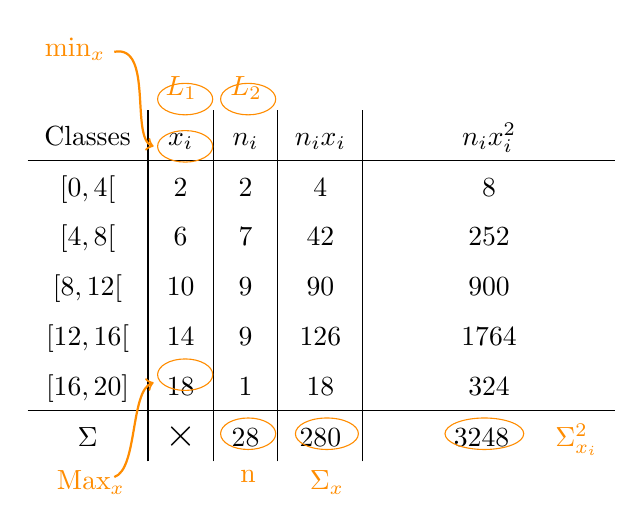
\begin{tikzpicture}

% Les deux lignes qui suivent servent au débogage
% \tikzstyle help lines=[color=blue!50,very thin] 
% \draw[help lines] (0,0) grid (8,6);

\begin{pgfonlayer}{background}

\node[line width=0.0pt,anchor=south west,rectangle,inner sep=0pt,outer sep=0pt]%
(Tbl) {%  A node must have a (possibly empty) label text.
\renewcommand{\arraystretch}{1.5}%
    \begin{tabular}{c|c|c|c|c}
\multicolumn{1}{c}{}& 
      \multicolumn{1}{c}{\textcolor{DarkOrange}{$L_1$}} & 
           \multicolumn{1}{c}{\textcolor{DarkOrange}{$L_2$}}  & \multicolumn{2}{c}{} \\
        Classes & $x_i$ & $n_i$ & $n_ix_i$ & $n_ix_i^2$ \\
      \hline
        $[0,4[$   & 2  & 2 & 4   & 8    \\
        $[4,8[$   & 6  & 7 & 42  & 252  \\
        $[8,12[$  & 10 & 9 & 90  & 900  \\
        $[12,16[$ & 14 & 9 & 126 & 1764 \\
        $[16,20]$ & 18 & 1 & 18  & 324  \\
     \hline
        $\Sigma$ & {\Large{$\times$}} & 28 & 280 & $\quad$ $\quad$ 3248
                    $\quad$ \textcolor{DarkOrange}{$\Sigma_{x_i}^2$} \\
    \end{tabular}
   };    
\end{pgfonlayer}

\begin{pgfonlayer}{foreground}
    \draw [color=DarkOrange](2,4.6)  circle  (.35 and .2); % Xi
    \draw [color=DarkOrange](2,4)  circle  (.35 and .2);   % 2
    \draw [color=DarkOrange](2.8,4.6)  circle  (.35 and .2); %Ni
    \draw [color=DarkOrange](2,1.1)  circle  (.35 and .2); %18
    \draw [color=DarkOrange](2.8,.35)  circle  (.35 and .2); %28
    \draw [color=DarkOrange](2.8,0)  node [below] {n} ; %28
    \draw [color=DarkOrange](3.8,.35)  circle  (.4 and .2); %280
    \draw [color=DarkOrange](3.8,0)  node [below] {$\Sigma_x$} ; %280
    \draw [color=DarkOrange](5.8,.35)  circle  (.5 and .2); %3248
    \draw [color=DarkOrange](.8,0)  node[below] {$\mathrm{Max}_x$} ;         
    \draw[->,line width=.8pt,DarkOrange]
          (1.1,-.2) .. controls +(0.3cm,.1cm) and +(-.3cm,-.1cm)..  
 %     node[below,label=\textcolor{blue}{$Max_x$}] {}
 %          node[below] {\textcolor{blue}{$Max_x$}}
     (1.6,1);
     \draw [color=DarkOrange](.6,5.5)  node[below] {$\mathrm{min}_x$} ;          
    \draw[->,line width=.8pt,DarkOrange]
   (1.1,5.2) .. controls +(0.5cm,.1cm) and +(-.3cm,.1cm).. (1.6,4);

\end{pgfonlayer}

\end{tikzpicture} 

\vspace*{.3cm}

$\overline{x} = \dfrac{\Sigma_{n_ix_i}}{\Sigma_{n_i}} = \dfrac{280}{28} = 10 $ \\

$\sigma_x = \sqrt{\overline{x^2} - \overline{x}^2} = \sqrt{\dfrac{3248}{28} - \left(\dfrac{280}{28}\right)^2} = \textcolor{DarkOrange}{\ovalbox{\textcolor{black}{4}}} \textcolor{DarkOrange}{\quad \sigma_x = 4}$ \\

\subsubsection{Répartition « normale »}

$\overline{x} - \sigma_x = 6$ \\
$\overline{x} + \sigma_x = 14$ \\

Interpolation linéaire : $ 0 + \dfrac{7 \times 2}{4} + 9 + \dfrac{9 \times 2}{4} + 0 = 17$ élèves, soit 60,71\%. \\

$2\overline{x} - 2\sigma_x = 2$ \\
$2\overline{x} + 2\sigma_x = 18$ \\

Interpolation linéaire : $ \dfrac{2 \times 2}{4} + 7 + 9 + 9 + \dfrac{1 \times 2}{4} \approx 26,5$ élèves, soit 94,64\%.

\newpage

\subsection{Exercice : Étude d'un caractère quantitatif continu}

Dans une maternité, on étudie la le poids des bébés en grammes pour 200 bébés. \\

On regroupe les bébés par classes d'amplitude 600. \\

On pose $X_i = \dfrac{1}{100}x_i$ \\

\begin{tabular}{c|c|c|c|c|c|c|c}
Classes & $n_i$ & $p_i$ & Pourcentages cumulés croissants & $x_i$ & $X_i$ & $n_iX_i$ & $n_iX_i^2$ \\
\hline
$[2000,2600[$ & 12 & 6 & 6 & 2300 & 23 & 276 & 6348 \\
$[2600,3200[$ & 64 & 32 & 38 & 2900 & 29 & 1856 & 53824 \\
$[3200,3800[$ & 84 & 42 & 80 & 3500 & 35 & 2940 & 102900 \\
$[3800,4400[$ & 38 & 19 & 99 & 4100 & 41 & 1558 & 63878 \\
$[4400,5000]$ & 2 & 1 & 100 & 4700 & 47 & 94 & 4418 \\
\hline
$\Sigma$ & 200 & 100 & {\Large {$\times$}} & {\Large {$\times$}} & {\Large {$\times$}} & 6724 & 231368 \\
\end{tabular}

\newpage


\subsubsection{Histogramme des pourcentages}

% \vspace*{.6cm}

\begin{center}

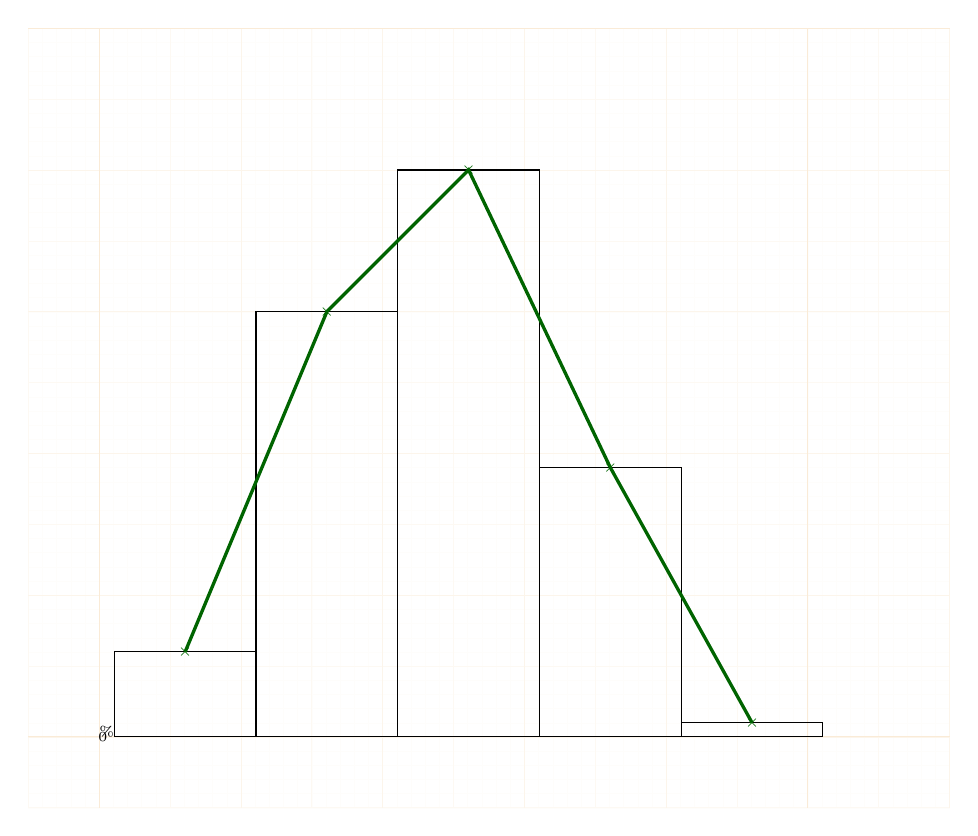
\begin{tikzpicture}[scale=1.8]
    \tikzstyle{AxeXStyle}=[>=latex’,->]
    \tikzstyle{AxeYStyle}=[-]
    \tkzInit[xmin=2000,xmax=5200,xstep=600,ymax=40,ystep=10]
    \tkzDrawX[label=$~$]
   \tkzLabelX[font=\tiny, color=black ]
    \tkzDrawY[label=$\%$]
    \tkzLabelY[orig=false, color=black ]  

\draw  
(0,0) node [left] {\textcolor{black}{0}} -- (0,.6) -- (1,.6) -- (1,0) -- (1,3) -- (2,3) -- (2, 0) -- (2, 4) 
-- (3, 4) -- (3,0) -- (3,1.9) -- (4,1.9) -- (4, 0) 
-- (4,.1) -- (5,.1) -- (5,0) -- cycle ; 
\draw [line width=1.2, color=DarkGreen] (.5,.6) node {$\times$} -- (1.5,3)node {$\times$} -- (2.5,4) node {$\times$} -- (3.5,1.9) node {$\times$} -- (4.5,.1) node {$\times$} ; 

\begin{pgfonlayer}{background}  
% Attention l'ordre de ces lignes est important 
% Ne pas le modifier   
\draw[step=1mm,ultra thin,AntiqueWhite!10](-.5,-.5)  grid (6,5);
\draw[step=5mm,very thin,AntiqueWhite!30] (-.5,-.5)   grid (6,5);
\draw[step=1cm,very thin,AntiqueWhite!50] (-.5,-.5)   grid (6,5);
\draw[step=5cm,thin,AntiqueWhite]         (-.5,-.5)  grid (6,5);
\end{pgfonlayer} 
\end{tikzpicture}
\end{center}

\subsubsection{Histogramme des pourcentages cumulés croissants}

% Inclure le dessin.
\begin{center}

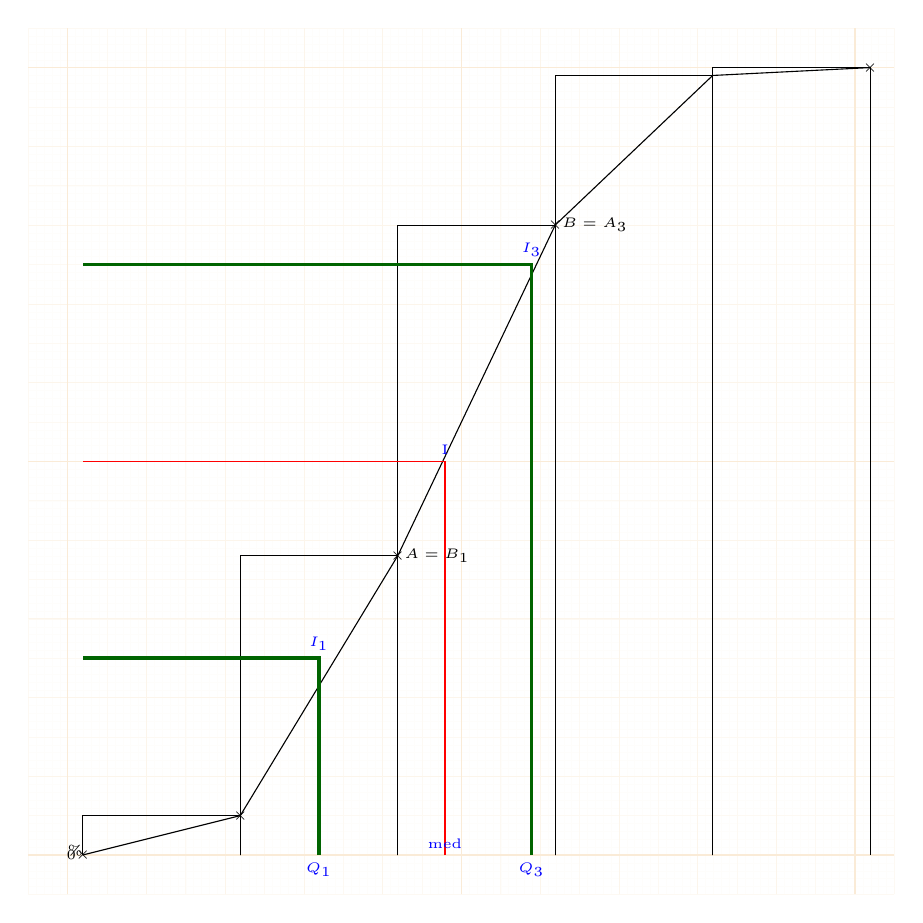
\begin{tikzpicture}[scale=1]
    \tikzstyle{AxeXStyle}=[>=latex’,->]
    \tikzstyle{AxeYStyle}=[-]
    \tkzInit[xmin=2000,xmax=5200,xstep=300,ymax=100,ystep=10]
    \tkzDrawX[label=$~$]
   \tkzLabelX[font=\tiny, color=black ]
    \tkzDrawY[label=$\%$]
    \tkzLabelY[orig=false, color=black ]  
\draw  (0,0) node {$\times$} -- (2,.5) node {$\times$} -- (4,3.8) node {$\times$} -- (6,8) node {$\times$} -- (8,9.9) --  (10,10.0) node {$\times$} ; 

\draw (0,0) node [left] {$0$} -- (0,.5) -- (2,.5) -- (2,0) 
-- (2,3.8) -- (4,3.8) node [right] {$A=B_1$} -- (4,0) -- (4,8) -- (6, 8) node [right] {$B=A_3$} -- (6,0) 
-- (6, 9.9) -- (8,9.9)  -- (8, 0) -- (8,10) -- (10,10) -- (10,0) ; 

\draw[color=DarkGreen,line width=1.2] (3,0) node [below] {\textcolor{blue}{$Q_1$}} 
    -- (3, 2.5) node [above] {\textcolor{blue}{$I_1$}} 
    -- (0, 2.5) ;  
    
\draw[color=red] (4.6,0) node [above] {\textcolor{blue}{med}} 
    -- (4.6, 5) node [above] {\textcolor{blue}{I}} 
    -- (0,5) ;    

\draw[color=DarkGreen,line width=1.2] (5.7,0) node [below] {\textcolor{blue}{$Q_3$}} 
    -- (5.7, 7.5) node [above] {\textcolor{blue}{$I_3$}} 
    -- (0, 7.5) ; 
         
\begin{pgfonlayer}{background}  
% Attention l'ordre de ces lignes est important 
% Ne pas le modifier   
\draw[step=1mm,ultra thin,AntiqueWhite!10](-.5,-.5)  grid (10.5,10.5);
\draw[step=5mm,very thin,AntiqueWhite!30] (-.5,-.5)  grid (10.5,10.5);
\draw[step=1cm,very thin,AntiqueWhite!50] (-.5,-.5)  grid (10.5,10.5);
\draw[step=5cm,thin,AntiqueWhite]         (-.5,-.5)  grid (10.5,10.5);
\end{pgfonlayer} 
\end{tikzpicture}
\end{center}

\newpage

Graphiquement, on lit : 

\begin{itemize}
\item[*] med $ \approx 3380$
\item[*] $Q_1 \approx 2960$ 
\item[*] $ Q_3 \approx 3710$ ou $3740$
\end{itemize} 

\vspace*{.3cm}

Par le calcul, on a : \\

\textbf{Médiane}

Avec les points $A(3200,38)$ $ B(3800,80)$, on peut opérer un changement d'unité. On utilisera donc les points $A'(32,48)$ et $B'(38,80)$. \\

Équation de la droite $(A'B')$ : $y=7X - 186$. \\

Intersection de $(A'B')$ et la droite $y=50$. \\

$7X - 186  = 50$ \\

$ 7X = 236$ \\

$ X = \dfrac{236}{7} \approx 33,71 $ \\

Donc med $= 3371$. 50\% des bébés pèsent moins de 3371 grammes et 50\% ont pèsent plus de 3371 grammes. \\

$\mathbf{Q_1}$  \\

Avec les points $A_1(2600,6)$ et $B_1(3200,38)$, on peut opérer un changement d'unité. On utilisera donc les points $A_1'(26,6)$ et $B_1'(32,38)$  \\

Équation de la droite $(A_1'B_1')$ : $y=\dfrac{16}{3}X - \dfrac{398}{3}$ \\

Intersection de $(A_1'B_1')$ et la droite $y=25$. \\

$ \dfrac{16}{3}X - \dfrac{398}{3} = 25$ \\

$ \dfrac{16}{3}X = \dfrac{473}{3} $ \\

$ X = \dfrac{473}{3} \times \dfrac{3}{16} = \dfrac{473}{16} $ \\

$ X \approx 29,56 $ \\

Donc $Q_1 = 2956$. \\

$\mathbf{Q_3}$ \\

Avec les points $A_3(3200,38)$ et $B_3(3800,80)$, on peut opérer un changement d'unité. On utilisera donc les points $A_3'(32,38)$ et $ B_3'(38,80)$. \\

Équation de la droite $(A_3'B_3')$ : $y= 7X -186 $.

Intersection de $(A_3'B_3')$ et la droite $y=75$. \\

$ 7X - 186 = 75 $ \\

$ 7X = 261 $ \\

$ X = \dfrac{261}{7} = 37,29 $ \\

$ X \approx 37,29 $ \\

Donc $Q_1 = 3729$. \\

Donc 50\% des bébés pèsent entre 2956 grammes et 3729 grammes.

\newpage

\subsubsection{Moyenne et écart-type}

$\overline{X} = \dfrac{\Sigma_{n_iX_i}}{\Sigma_{n_i}} = \dfrac{6724}{200} = 33,62. $ \\

Donc $\overline{x} = 3362$ grammes. \\

$\sigma_X = \sqrt{\overline{x^2} - \overline{x}^2} = \sqrt{\dfrac{231368}{200} - \left(\dfrac{6724}{200}\right)^2} \approx = 5,15$. \\

Donc $ \sigma _x = 5,15$ grammes. \\

\subsubsection{Répartition normale}

$\overline{x} - \sigma_x = 2847$ \\
$\overline{x} + \sigma_x = 3877$ \\

Interpolation linéaire : $ 0 + \dfrac{64 \times 353}{600} + 84 + \dfrac{38 \times 77}{600} + 0 = 126,53$ bébés, soit 63,27\%. \\

$2\overline{x} - 2\sigma_x = 2332$ \\
$2\overline{x} + 2\sigma_x = 4392$ \\

Interpolation linéaire : $ \dfrac{\dfrac{12 \times 268}{600} + 64 + 84 + \dfrac{38 \times 592}{600}}{200} \times 100 = 95,43$\%. \\

\newpage

\subsection{Amusette : Effet de structure}

Attention aux pièges des moyennes.

Dans un premier centre d'examen, on a $\overline{x_{1_G}}$ la moyenne des garçons, et $\overline{x_{1_F}}$ la moyenne des filles. Dans un seconde centre, on a $\overline{x_{2_G}}$ et $\overline{x_{2_F}}$ la moyenne des filles. \\

On donne : $\overline{x_{1_G}} = 13$ et $\overline{x_{1_F}} = 12$. \\

De plus, on a : $\overline{x_{2_G}} = 9 $ et $\overline{x_{2_F}} = 8$. \\

Peut-on dire que les garçons sont meilleurs que les filles ?

Dans le premier centre d'examen, il y a 58 garçons et 104 filles. \\
Dans le second centre d'examen, il y a 87 garçons et 32 filles. \\

On calcule $\overline{x_G}$, la moyenne générale des garçons : \\

$\dfrac{58 \times 13 + 87 \times 9}{58 + 87} = 10,60 $ \\

Puis, on calcule $\overline{x_F}$, la moyenne générale des filles : \\

$ \dfrac{12 \times 104 + 8 \times 32 }{104 + 32} = 11,06 $. \\

Finalement, les filles sont meilleures que les garçons.
